% Options for packages loaded elsewhere
\PassOptionsToPackage{unicode}{hyperref}
\PassOptionsToPackage{hyphens}{url}
%
\documentclass[
]{article}
\usepackage{amsmath,amssymb}
\usepackage{lmodern}
\usepackage{ifxetex,ifluatex}
\ifnum 0\ifxetex 1\fi\ifluatex 1\fi=0 % if pdftex
  \usepackage[T1]{fontenc}
  \usepackage[utf8]{inputenc}
  \usepackage{textcomp} % provide euro and other symbols
\else % if luatex or xetex
  \usepackage{unicode-math}
  \defaultfontfeatures{Scale=MatchLowercase}
  \defaultfontfeatures[\rmfamily]{Ligatures=TeX,Scale=1}
\fi
% Use upquote if available, for straight quotes in verbatim environments
\IfFileExists{upquote.sty}{\usepackage{upquote}}{}
\IfFileExists{microtype.sty}{% use microtype if available
  \usepackage[]{microtype}
  \UseMicrotypeSet[protrusion]{basicmath} % disable protrusion for tt fonts
}{}
\makeatletter
\@ifundefined{KOMAClassName}{% if non-KOMA class
  \IfFileExists{parskip.sty}{%
    \usepackage{parskip}
  }{% else
    \setlength{\parindent}{0pt}
    \setlength{\parskip}{6pt plus 2pt minus 1pt}}
}{% if KOMA class
  \KOMAoptions{parskip=half}}
\makeatother
\usepackage{xcolor}
\IfFileExists{xurl.sty}{\usepackage{xurl}}{} % add URL line breaks if available
\IfFileExists{bookmark.sty}{\usepackage{bookmark}}{\usepackage{hyperref}}
\hypersetup{
  pdftitle={THE FANDOMS OF THE NBA},
  pdfauthor={Philipp Kläger},
  hidelinks,
  pdfcreator={LaTeX via pandoc}}
\urlstyle{same} % disable monospaced font for URLs
\usepackage[margin=1in]{geometry}
\usepackage{graphicx}
\makeatletter
\def\maxwidth{\ifdim\Gin@nat@width>\linewidth\linewidth\else\Gin@nat@width\fi}
\def\maxheight{\ifdim\Gin@nat@height>\textheight\textheight\else\Gin@nat@height\fi}
\makeatother
% Scale images if necessary, so that they will not overflow the page
% margins by default, and it is still possible to overwrite the defaults
% using explicit options in \includegraphics[width, height, ...]{}
\setkeys{Gin}{width=\maxwidth,height=\maxheight,keepaspectratio}
% Set default figure placement to htbp
\makeatletter
\def\fps@figure{htbp}
\makeatother
\setlength{\emergencystretch}{3em} % prevent overfull lines
\providecommand{\tightlist}{%
  \setlength{\itemsep}{0pt}\setlength{\parskip}{0pt}}
\setcounter{secnumdepth}{-\maxdimen} % remove section numbering
\usepackage{booktabs}
\usepackage{booktabs}
\usepackage{longtable}
\usepackage{array}
\usepackage{multirow}
\usepackage{wrapfig}
\usepackage{float}
\usepackage{colortbl}
\usepackage{pdflscape}
\usepackage{tabu}
\usepackage{threeparttable}
\usepackage{threeparttablex}
\usepackage[normalem]{ulem}
\usepackage{makecell}
\usepackage{xcolor}
\ifluatex
  \usepackage{selnolig}  % disable illegal ligatures
\fi

\title{THE FANDOMS OF THE NBA}
\author{Philipp Kläger}
\date{}

\begin{document}
\maketitle
\begin{abstract}
The analysis revealed that the sentiments and emotions towards different
NBA teams are not only different, but also ambivalent in its direction.
There are no teams that are ``purely'' perceived in a negative or
positive manner. This observation is accurate for every team except for
the three franchises that didn't induce any significant Exemplary for
this, the LA Lakers are the most ``hated'' franchise in this sample, yet
they are also unlikely to be perceived in combination with angry or sad
feelings. Recent success seems to be an important factor how teams are
perceived on Twitter. Given this implication, marketers should exploit
recent success in the league with their marketing campaigns to exploit
this - for example after a big playoff win.
\end{abstract}

\hypertarget{i.-introduction}{%
\subsubsection{I. Introduction}\label{i.-introduction}}

``Sport has the power to change the world. It has the power to inspire,
it has the power to unite people in a way that little else does.`` -
Nelson Mandela, human rights activist (Rigney 2020)

Why do people love sports so much? On a personal level, most people will
probably have a different answer to this question. According to sports
psychologists, there are a total of eight different motivations. Being
exciting and aesthetically pleasing are among the most frequently
occurring reasons, but people also seek self-esteem benefits, money
interests, joint experience with family members or loved ones, as well
as because it offers a venue for emotional expression (Wann et. al.,
2001; Simons 2014).

As the NBA playoffs have recently started, I have decided to explore the
sentiments and emotions in the fandoms of the NBA. Subsequently, this
research seeks to present a descriptive analysis about sentiments
towards different NBA teams on Twitter and which factors influence these
sentiments.

\hfill\break

\hypertarget{ii.-literature-review-related-work-industry-background}{%
\subsubsection{II. Literature Review: Related Work \& Industry
Background}\label{ii.-literature-review-related-work-industry-background}}

``Our collective success has forged some kind of unity in this huge and
normally fragmented metropolis, it cuts across cultural and class
lines.`` - Kareem Abdul-Jabbar, NBA Hall of Famer about the LA Lakers
(Zhang et. al., 2018)

Considering the immense interest in sports and their fans, there is
surprisingly little research on fan behavior and its respective
emotions. Subsequently, this research intends to add to the already
existing scenery of empirical studies with an exploratory analysis of
sentiments and emotions towards different NBA teams. To provide an
extensive and detailed foundation for this endeavor, this review will
synthesize the current status of research regarding the sentiments and
emotions towards sports teams, as well provide an industry background
regarding the characteristics and possible differences between current
NBA teams and its supporters.

\hfill\break

\hypertarget{related-work}{%
\paragraph{Related Work}\label{related-work}}

While all sorts of fandom can be characterized as overall positive,
research indicates that sentiments and levels of engagement towards
different teams vary depending on a set of factors such as the
respective team's success. A recently conducted sentiment analysis of
comments in NBA-related communities suggests that fans of top teams are
more active in surprising losses, as fans of lower-seeded teams are more
active in surprising wins. They also discovered empirical evidence for a
phenomenon commonly referred to as ``bandwagon fans,'' which represents
the coherence between strong team performance and a significantly larger
share of fans with low loyalty (Zhang et. al., 2018). Further research
about the football 2014 World Cup displays that positive (anticipation
\& joy) and negative (fear \& anger) fan reactions were consistent with
goal results, while also indicating different levels of sentiments
depending on the team allegiances, as non-US game sample showed more
positive reactions than the main sample (Yu \& Wang 2014).

\hfill\break

\hypertarget{industry-background}{%
\paragraph{Industry Background}\label{industry-background}}

As can be expected, NBA fandom is often dependent on a supporter's
location. Within proximity to the home city of a team, usually, the most
supporters can be found. This is especially visible in the most crowded
area of NBA teams in the southwest of the US, where six teams are
situated close by. However, there are several exceptions. The most
successful teams of the past two decades, the Los Angeles Lakers and San
Antonio Spurs (won five championships each since 2000) have managed to
find supporters all over the country, indicating that success is a big
factor for people in choosing their allegiances. The Toronto Raptors
managed to persuade the vast majority of Canada, which can be attributed
to a potentially higher degree of national loyalty in fandom in Canada
(Twitter Blog 2015).

\begin{figure}

{\centering 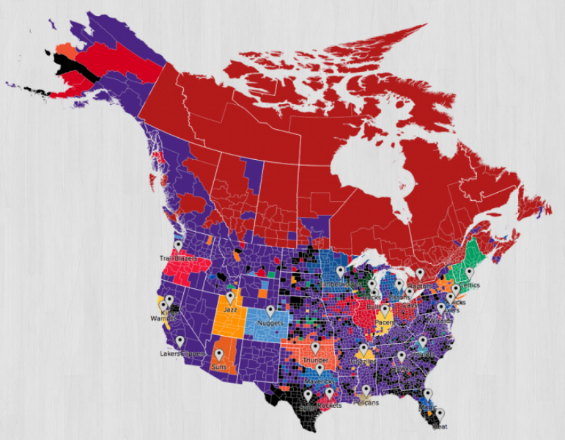
\includegraphics[width=7.85in,height=0.4\textheight]{../output/Figure 1 - NBA Fandoms Map (Twitter Blog 2015)} 

}

\caption{Fandom Allegiances: most liked NBA teams per county ;Source: Twitter Blog (2015)}\label{fig:unnamed-chunk-2-1}
\end{figure}
\begin{figure}

{\centering 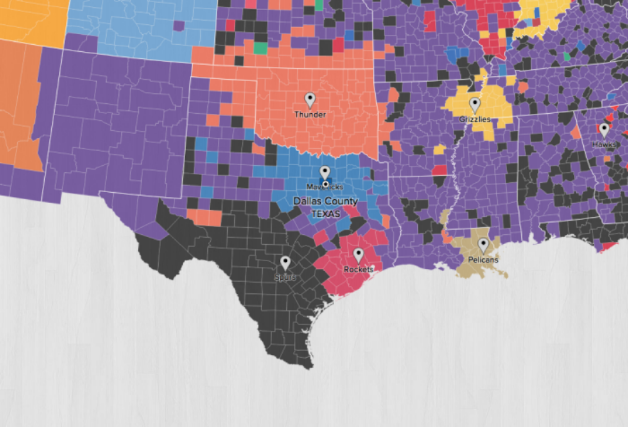
\includegraphics[width=8.72in,height=0.4\textheight]{../output/Figure 2 - NBA Fandoms Map Southwest (Twitter Blog 2015)} 

}

\caption{Fandom Allegiances: most liked NBA teams per county ;Source: Twitter Blog (2015)}\label{fig:unnamed-chunk-2-2}
\end{figure}

Recent research suggests that regarding sentiments and emotions,
(recent) success can be the source of both allegiance and resentment
towards NBA teams. This can be perfectly visualized with the example of
the Brooklyn Nets: they had been hardly discussed at the time of the
Twitter Blog study (2015) due to their lack of success and no
championship aspirations. Yet they also have quickly emerged as the most
hated team in the entire league arguably due to their recent success
this year with championship aspirations -- they experienced an increase
of their winning percentage from 46.3\% to 66.7\%. Additionally, with
traditional rivalries, the study suggests another reason for resenting
specific teams, as the Boston Celtics are mostly hated in Pennsylvania,
the home of their arch-rival, the Philadelphia 76ers (BasketballNews
2021; Basketball-Reference 2021).

\begin{figure}

{\centering 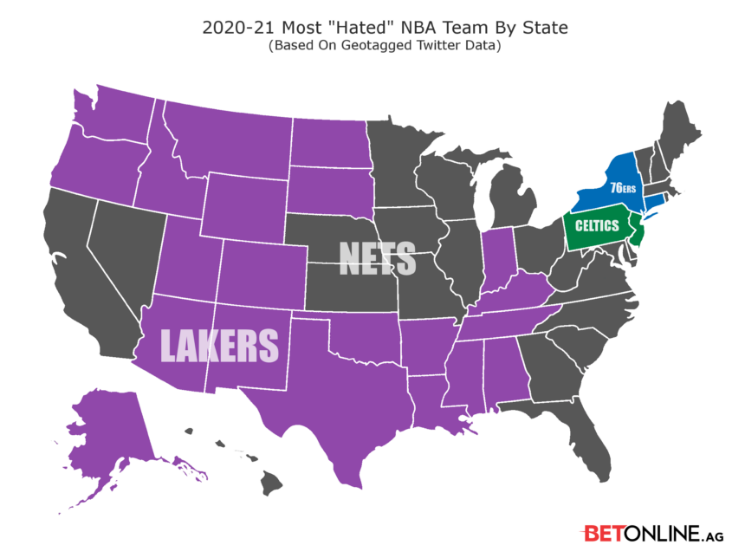
\includegraphics[width=10.35in,height=0.4\textheight]{../output/Figure 3 - 2020-21 Most Hated NBA Team By State (BasketballNews 2021)} 

}

\caption{Resentment: most hated NBA teams per state; Source: BasketballNews.com (2021)}\label{fig:unnamed-chunk-3}
\end{figure}

In recent years, there has been an interesting development regarding
teams that haven't enjoyed as much success as storied franchises. On
Twitter, smaller teams like the Atlanta Hawks or Portland Trail Blazers
have exercised a remarkably larger engagement on social media, as their
official accounts initiated the most conversations among NBA-related
tweets. This is surprising, because they are among the teams with the
lowest number of followers, whereas the Lakers, the leader in followers,
initiate the least amount of Twitter conversations. This could be an
indication that smaller teams try to outweigh the lack of success with a
higher degree of engagement on social media to attract fans.

\begin{figure}

{\centering 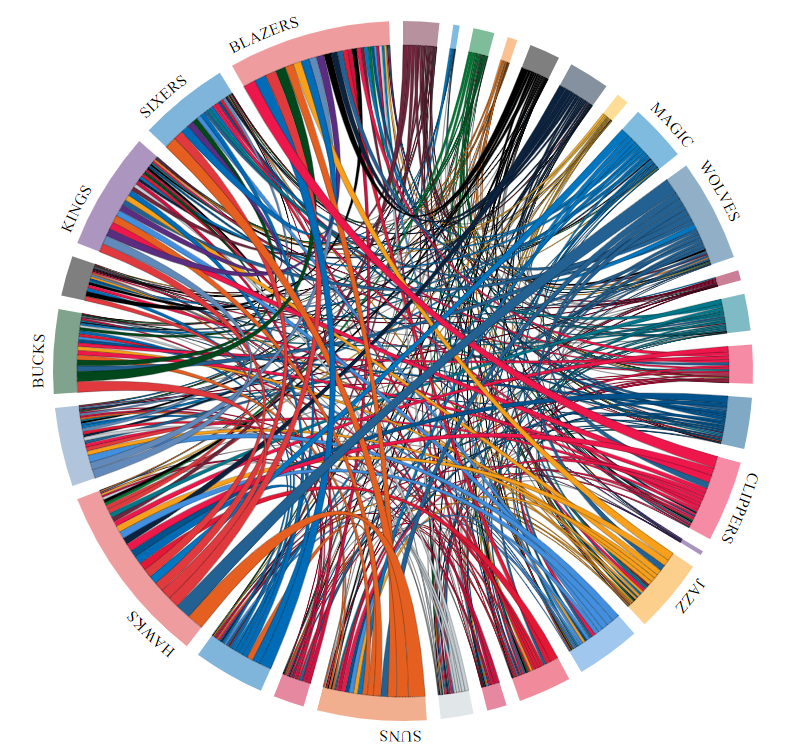
\includegraphics[width=11.19in,height=0.4\textheight]{../output/Figure 4 - Relationships & Conversations by official Twitter accounts of NBA teams (Capital News Service 2018)} 

}

\caption{Number of initiated conversations; Sources: Capital News Service (2018) / Statista (2021)}\label{fig:unnamed-chunk-4}
\end{figure}

\hfill\break

\hypertarget{iii.-data}{%
\subsubsection{III. Data}\label{iii.-data}}

\hypertarget{data-collection}{%
\paragraph{Data Collection}\label{data-collection}}

The data was collected from Twitter on March 20th 2021 with the Twitter
Search API. The initial data set contained 10716 observations and 50
variables. A file with the names of all 30 NBA teams in form of hashtags
was utilized to identify and access the adequate data from the platform.

\hfill\break

\hypertarget{data-processing}{%
\paragraph{Data Processing}\label{data-processing}}

After examining the data, multiple data cleaning and preparation actions
were necessary. Firstly, unnecessary columns for the analysis were
dropped. Secondly, a set of team id variables were created to assign
each tweet to the mentioned team. This was accomplished with first
creating an index variable, that detected each team assignment to a
specific number (e.g., Brooklyn Nets with 3). Afterwards, a dummy
variable was created for each team, indicating the value 1 if the team
was indeed mentioned and 0 for every other team. Thirdly, tweets that
could not be assigned to a team and missing values were erased, which
reduced the number of observations to 9714. Lastly, the text data was
cleaned to prepare the analysis appropriately by removing links,
mentions, htmls, numbers, excess whitespaces and unneeded special
characters.

\begin{figure}

{\centering \includegraphics[width=50.53in,height=0.4\textheight]{../output/SummaryTable} 

}

\caption{Sample Overview}\label{fig:unnamed-chunk-5}
\end{figure}

\hfill\break

\hypertarget{iv.-methodology}{%
\subsubsection{IV. Methodology}\label{iv.-methodology}}

\hypertarget{sentiment-analysis}{%
\paragraph{Sentiment Analysis}\label{sentiment-analysis}}

The sentiment analysis of this research was conducted with the
syuzhet-package and the NRC Word-Emotion Association Lexicon. The NRC
Lexincon refers to a list of English words that displays their
respective associations to eight basic emotions (anger, fear,
anticipation, trust, surprise, sadness, joy and disgust) and two
sentiments (negative and positive). The associations were crafted manual
with the means of crowdsourcing (Mohammad 2021).

\hfill\break

\hypertarget{linear-regressions}{%
\paragraph{Linear Regressions}\label{linear-regressions}}

After running the sentiment analysis, a series of linear regressions
were conducted to determine which sentiments and emotions to each team.
For each regression, the NBA team id was the dependent variables for the
variables attained in the sentiment analysis.

\hfill\break

\hypertarget{v.-results}{%
\subsubsection{V. Results}\label{v.-results}}

The analysis yields multiple interesting insights:

\begin{itemize}
\item
  The Los Angeles Lakers are significantly linked to multiple sentiments
  and emotions. They are most likely to be brought up in negative
  tweets, yet surprisingly least likely to be linked to tweets including
  anger or sadness sentiments.
\item
  The Phoenix Suns are most likely to be mentioned in a positive
  sentiment tweet, but also least likely to be tagged in tweets that
  issue trust.
\item
  The Chicago Bulls are most likely to be mentioned in tweets with joy
  or surprise, yet least likely to be named in a tweet about
  anticipation.
\item
  The Sacramento Kings are most likely to be tagged in a tweet embodying
  trust or sadness, however they are least likely to be included in a
  tweet about fear or with positive sentiment.
\item
  The franchises of Memphis Grizzlies, Houston Rockets and Philadelphia
  76ers did not display any significant connection to any sentiment or
  emotion, which may indicate that the social media presence of their
  official team account and their respective fans do not post many
  emotionally driven tweets.
\end{itemize}

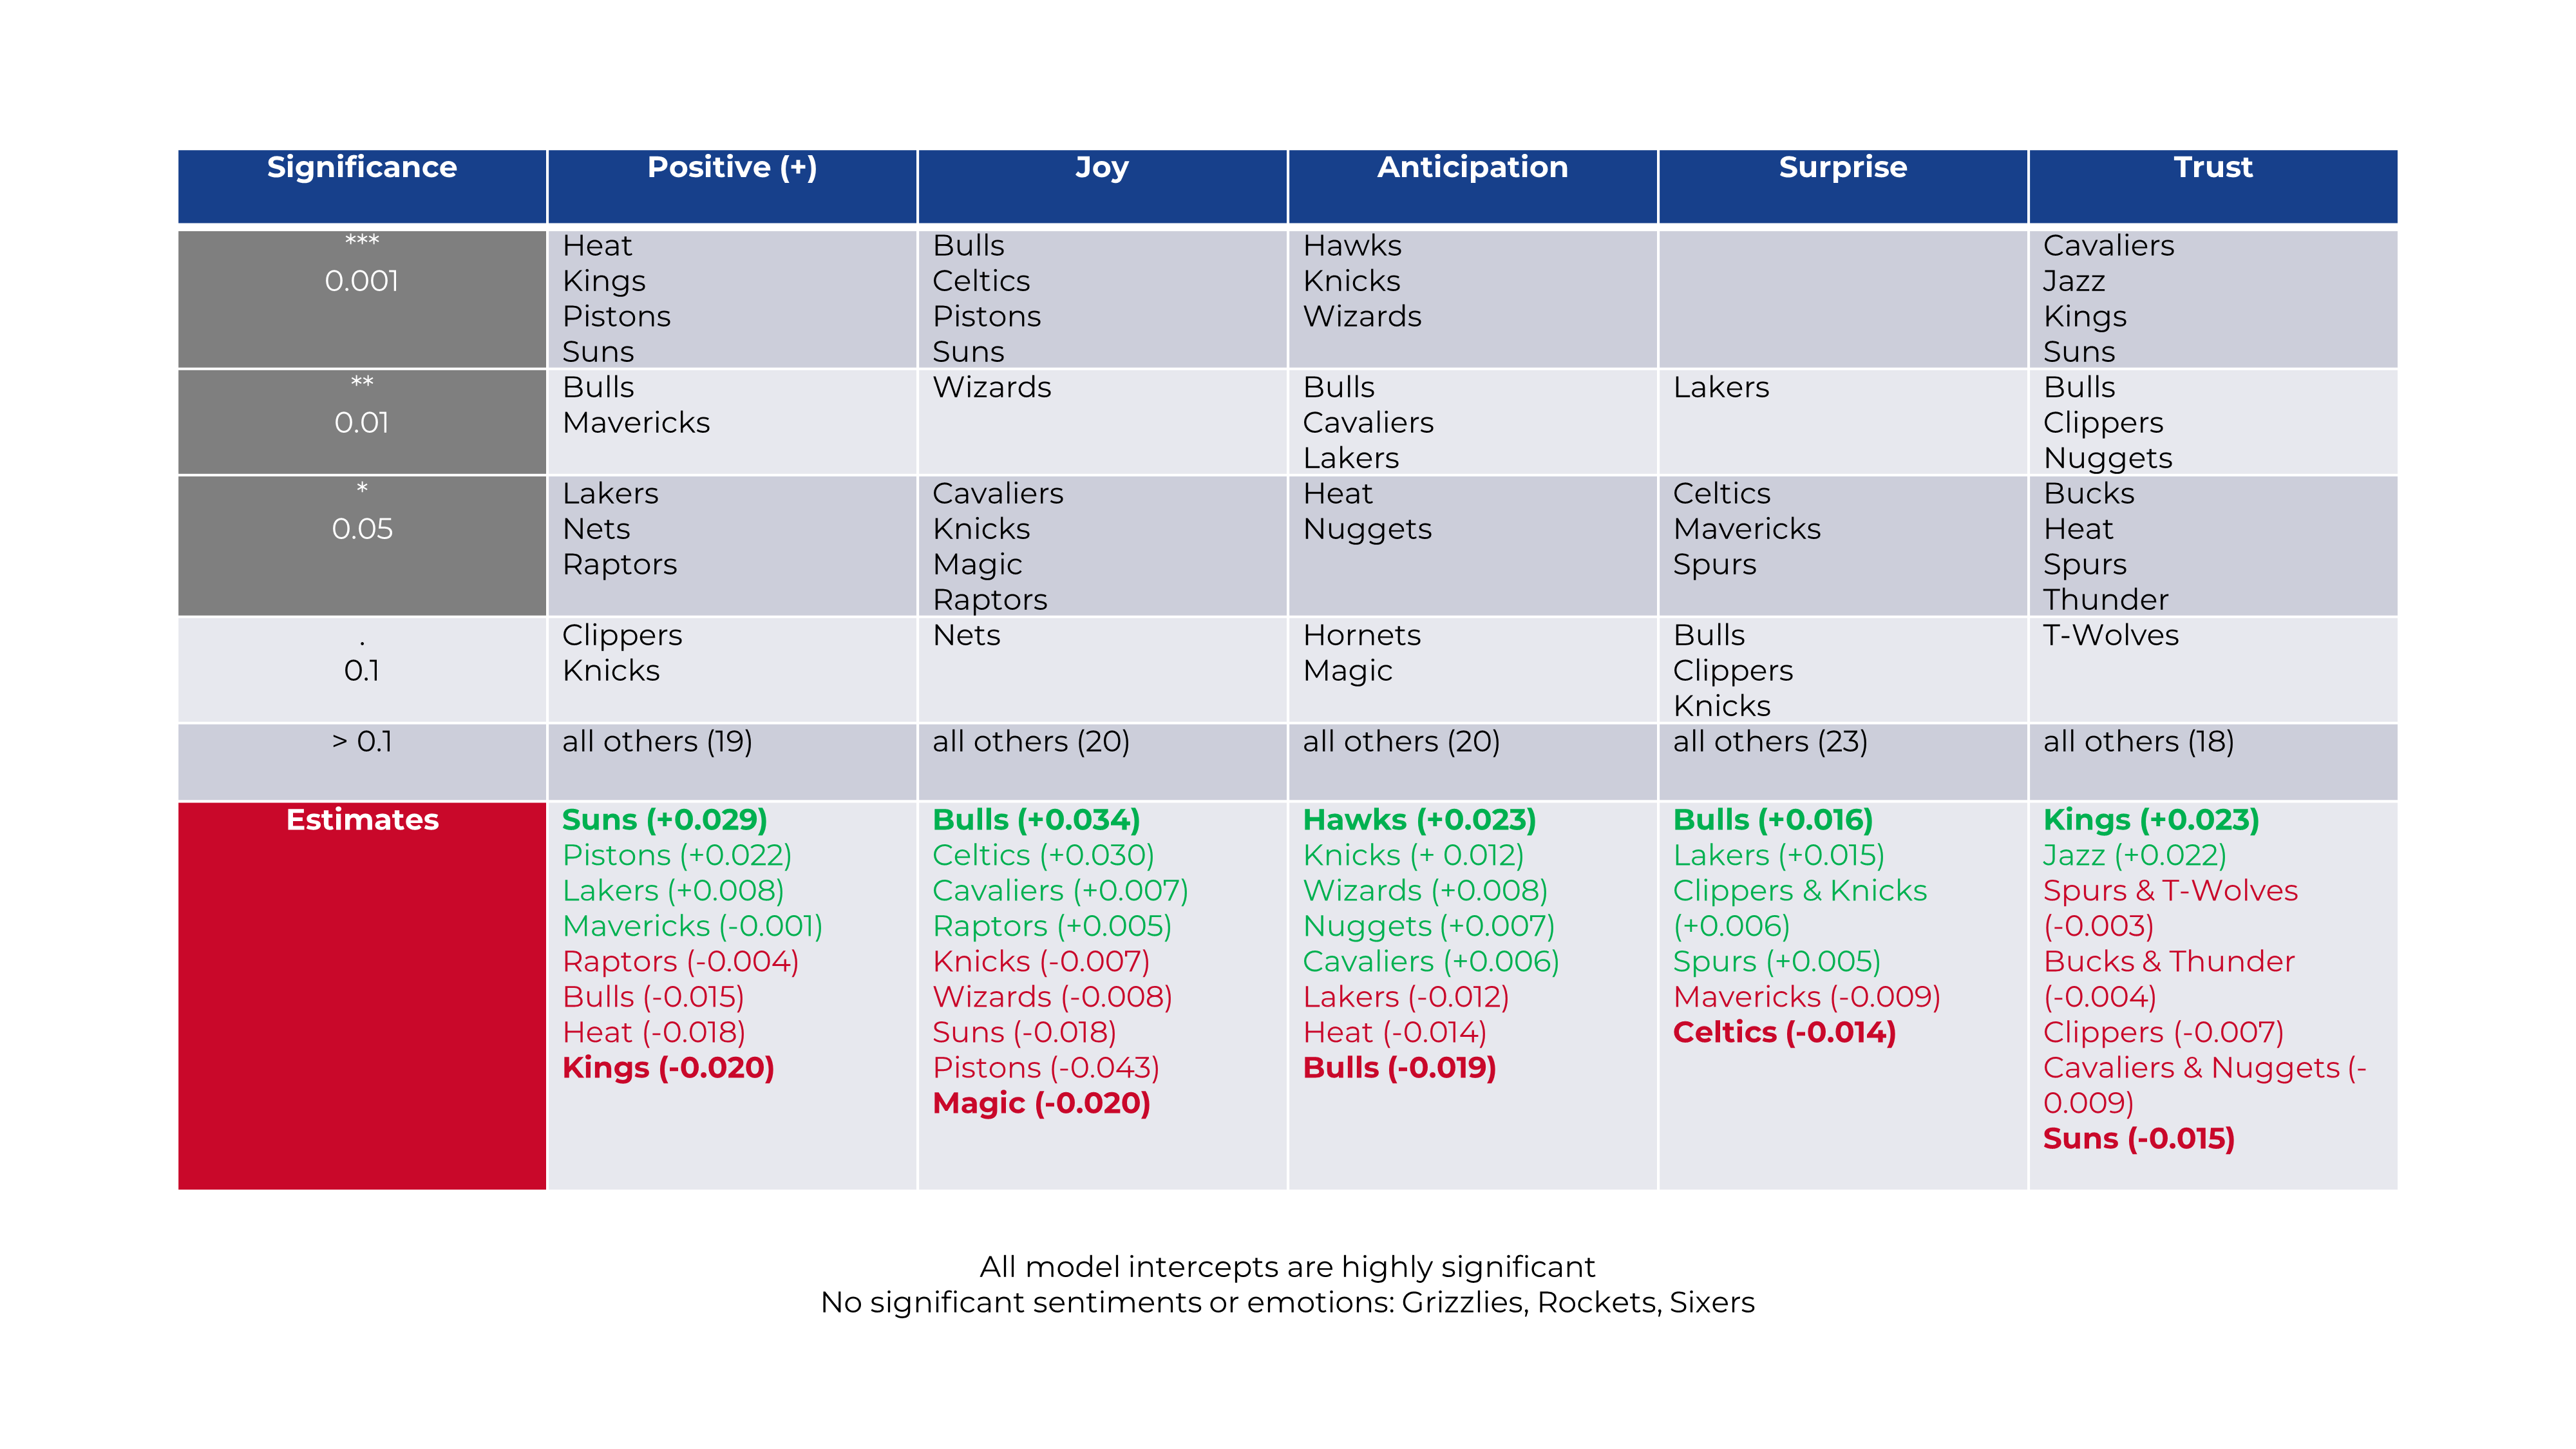
\includegraphics[width=55.56in]{../output/Positive Sentiments & Emotions}
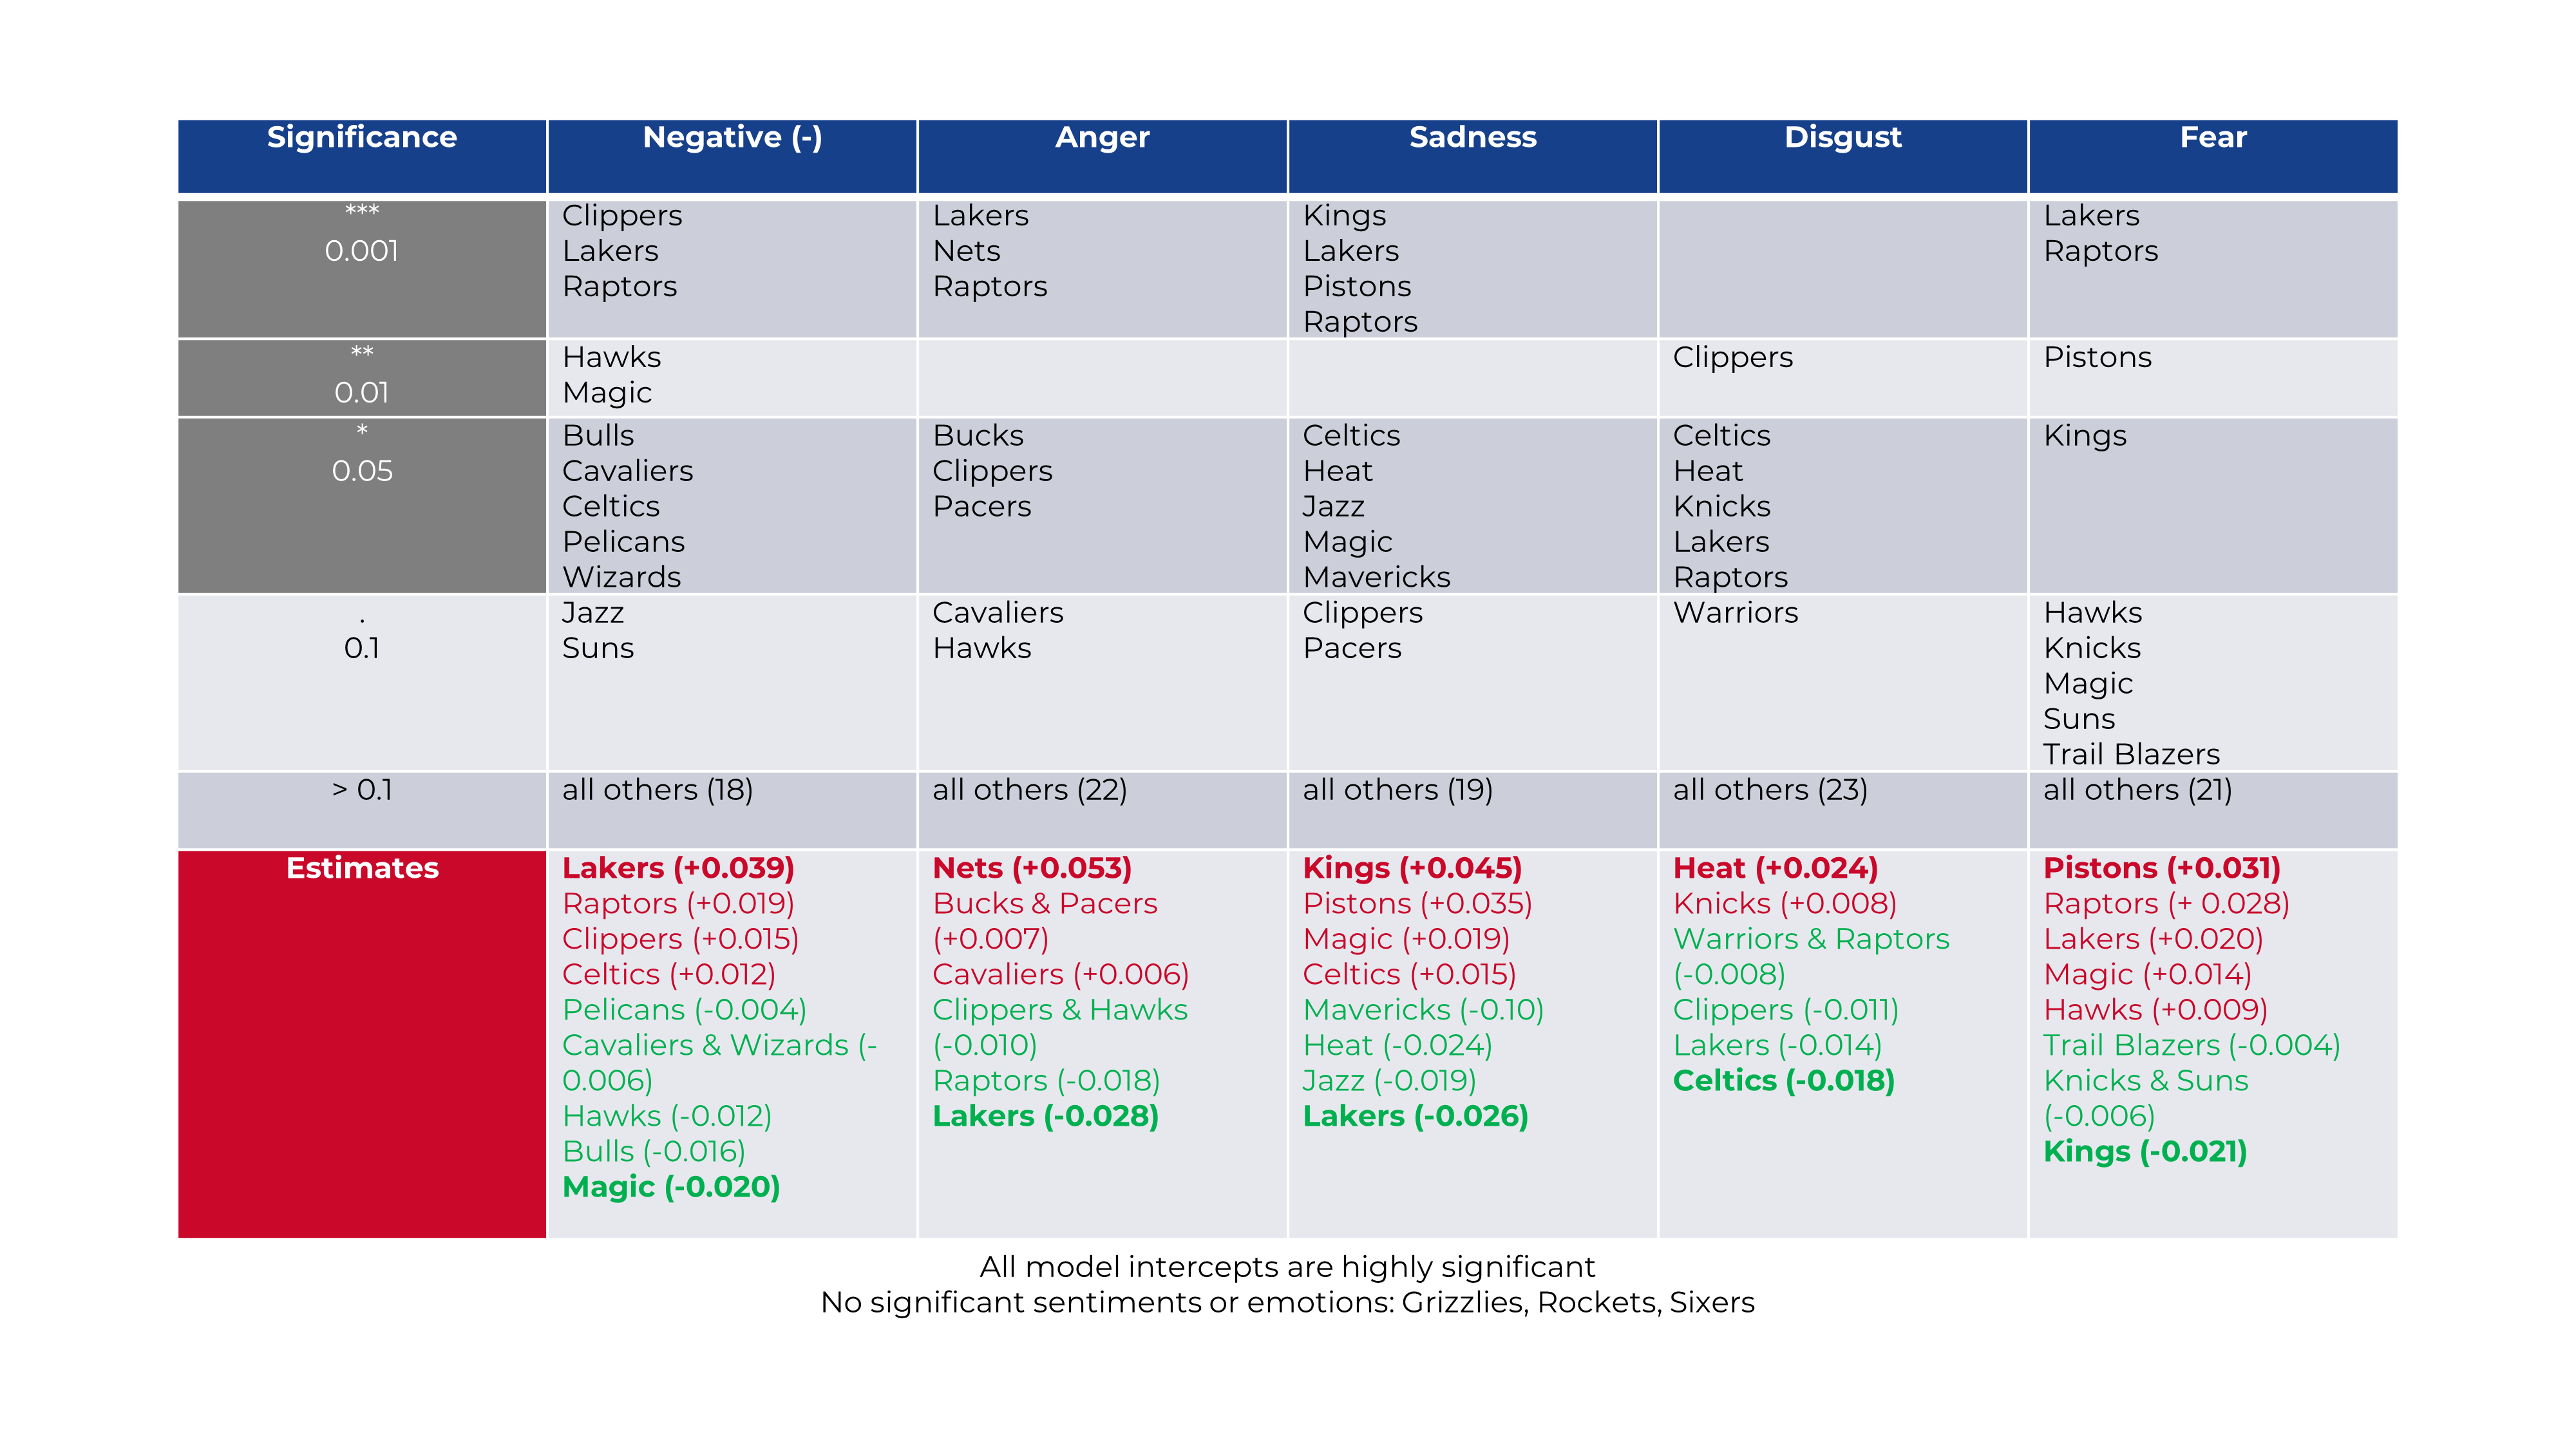
\includegraphics[width=55.56in]{../output/Negative Sentiments & Emotions}

\hfill\break

\hypertarget{vi.-discussion-conclusion}{%
\subsubsection{VI. Discussion \&
Conclusion}\label{vi.-discussion-conclusion}}

The analysis revealed that the sentiments and emotions towards different
NBA teams are not only different, but also ambivalent in its direction.
There are no teams that are ``purely'' perceived in a negative or
positive manner. This observation is accurate for every team except for
the three franchises that didn't induce any significant Exemplary for
this, the LA Lakers are the most ``hated'' franchise in this sample, yet
they are also unlikely to be perceived in combination with angry or sad
feelings.

\hypertarget{managerial-relevance}{%
\paragraph{Managerial Relevance}\label{managerial-relevance}}

Recent success seems to be an important factor how teams are perceived
on Twitter. Given this implication, marketers should exploit recent
success in the league with their marketing campaigns to exploit this -
for example after a big playoff win.

\hypertarget{future-directions-of-research}{%
\paragraph{Future Directions of
Research}\label{future-directions-of-research}}

Given the relatively small scope and sample size, future research might
attain more detailled implications and results with a larger time frame
of observations, as this research only included the tweets about the NBA
teams of one week.

\hfill\break

\hypertarget{word-count}{%
\paragraph*{Word Count}\label{word-count}}
\addcontentsline{toc}{paragraph}{Word Count}

Number of Words: 1788

\hypertarget{references}{%
\subsubsection{References}\label{references}}

Almendrala, A. (2017): How Being A Sports Fan Makes You Happier and
Healthier, in: The Huffington Post. Retrieved from:
\url{https://www.huffpost.com/entry/sports-fan-mental-health-benefits_n_6565314}

BasketballNews (2021, May 22nd): Study: Who's the most hated team in the
NBA right now? Retrieved from:
\url{https://www.basketballnews.com/stories/study-whos-the-mosthated-team-in-the-nba-right-now}

Basketball-Reference (2021): Brooklyn Nets. Retrieved from:
\url{https://www.basketball-reference.com/teams/NJN/}

Bernhardt, P.C., Dabbs Jr., J.R., Fielden, F.A. \& Lutter, C.D. (1998):
Testosterone changes during vicarious experiences of winning and losing
among fans at sporting events, in: Physiological Behavior, 65(1).

Capital News Service (2018, June 3rd): The hidden Twitter relationships
of NBA teams. Retrieved from:
\url{https://cnsmaryland.org/2018/06/03/the-relationships-between-nba-teams-twitter-accounts/}

Mohammad, S. (2021): NRC Word-Emotion Association Lexicon. Retrieved
from: \url{https://saifmohammad.com/WebPages/NRC-Emotion-Lexicon.htm}

Rigney, R. (2020, February 12th): Why do we love sports?, in: PSU
Vanguard. Retrieved from:
\url{https://psuvanguard.com/why-do-we-love-sports/}

Simons, E. (2014): What science can tell sportswriters about why we love
sports, in: Columbia Journalism Review. Retrieved from:
\url{https://archives.cjr.org/full_court_press/science_sportswriting.php}

Statista (2021): Twitter followers of NBA teams as of March 2021.
Retrieved from:
\url{https://www.statista.com/statistics/240386/twitter-followers-of-national-basketball-association-teams/}

Twitter Blog (2015): \#NBA fans: Where are your team's followers?
Retrieved from:
\url{https://blog.twitter.com/en_us/a/2015/nba-fans-where-are-your-team-s-followers}

Wang, Y. \& Zhou S. (2015): How do sports organizations use social media
to build relationships? A content analysis of NBA clubs' Twitter use,
University of Alabama, 1-65.

Wann, D.L., Melnick, M.J., Russell, G.W. \& Pearse, D.G. (2001): Sport
Fans: The psychology and social impact of spectators, Routledge.

Yu Y. \& Wang X. (2014): World Cup 2014 in the Twitter World: A big data
analysis of sentiments in U.S. fans' tweets, in: Computers in Human
Behavior, Vol. 48, 392-400.

Zhang, J.S., Tan, C. \& Lv, Q. (2018): ``This why we play'':
Characterizing Online Fan Communities of the NBA Teams, in: Proceedings
of the ACM on Human-Computer Interaction, CSCW, Art. 197, 1-25.

\end{document}
